\documentclass[11pt]{article}
\usepackage[utf8]{inputenc}\usepackage[T1]{fontenc}
\usepackage{amsmath,amssymb,amsthm}\usepackage[margin=1in]{geometry}
\usepackage{graphicx}\usepackage{booktabs}
\usepackage[hidelinks]{hyperref}

\title{Cousin and Sexy Prime Pairs on the $6N$ Skeleton:\\
Three $\omega$-Distortions Set by Pairing Geometry}
\author{Ruqing Chen\\
\small GUT Geoservice Inc., Montreal, Quebec, Canada\\
\small \texttt{ruqing@hotmail.com}}
\date{\today}

\begin{document}
\maketitle

\begin{abstract}
Parts~I--VIII built a conditional theory of twin pairs $(6N{-}1,6N{+}1)$ on the
$6N$ skeleton, in which the pair rate rises sharply with the factor count
$\omega_{>3}(N)$ of the single shared centre. Here we ask whether the same
$\omega$-dependence carries over to cousin pairs (difference $4$) and sexy pairs
(difference $6$). It does not carry over identically; instead it distorts into
three distinct, geometry-determined shapes. On the $6N$ skeleton a cousin pair is
$(6N{+}1,\,6(N{+}1){-}1)$ and a sexy pair is either
$(6N{-}1,\,6(N{+}1){-}1)$ (``sexy-A'') or $(6N{+}1,\,6(N{+}1){+}1)$ (``sexy-B'');
unlike the twin, all of these straddle two consecutive centres $N$ and $N{+}1$.
Binning by the left centre's $\omega$ on the $1.5\times10^{9}$ centres of $S_{10}$
(over $5\times10^{8}$ pairs), we find: the twin rate rises monotonically (to
$4.8\times$ at $\omega=7$); the cousin and sexy-A rates fall monotonically (to
$0.13$--$0.15\times$) and are numerically identical to three decimals at every
$\omega$; and the sexy-B rate is non-monotone, peaking near $\omega=4$ before
falling. The cousin/sexy-A coincidence is explained by their shared right member
$6(N{+}1){-}1$. The single-centre enrichment of the twin thus reverses or becomes
non-monotone once the pair straddles two centres, with the sign of the distortion
fixed by which wings are involved. We give the phenomenon and its geometric
account; a quantitative two-centre mechanism is posed as the open problem. No
claim is made about the infinitude of any prime constellation.
\end{abstract}

\section{Geometry of the pairs}

On the $6N$ skeleton (all primes $>3$ lie on $6N\pm1$) the three constellations
take fixed forms. A twin pair is $(6N{-}1,6N{+}1)$, the two wings of a
\emph{single} centre $N$. A cousin pair (difference $4$) must be
$(6N{+}1,\,6N{+}5)=(6N{+}1,\,6(N{+}1){-}1)$, since the alternative $6N{+}3$ is
always divisible by $3$; it straddles centres $N$ and $N{+}1$ (right wing of $N$,
left wing of $N{+}1$). A sexy pair (difference $6$) is either
\[
  \text{sexy-A: }(6N{-}1,\,6(N{+}1){-}1)\quad\text{or}\quad
  \text{sexy-B: }(6N{+}1,\,6(N{+}1){+}1),
\]
both straddling $N$ and $N{+}1$ (two left wings, or two right wings,
respectively). The essential contrast: the twin lives on one centre, while
cousin and sexy live on two consecutive centres. The conditional theory of
Parts~I--VIII attributes a pair to a centre's factor count $\omega_{>3}$; for the
straddling pairs we attribute to the \emph{left} centre $N$, the natural analogue.

\section{Three distortions in $S_{10}$}

We scan all $1.5\times10^{9}$ centres of $S_{10}$ ($6N\in[10^9,10^{10})$),
determine $\omega_{>3}(N)$ and the primality of both wings of every centre, and
count each constellation binned by the left centre's $\omega$
(Table~\ref{tab:cs}, Fig.~\ref{fig:cs}). Rates are normalised to $\omega=1$ to
compare shapes.

\begin{table}[h]\centering\small
\begin{tabular}{rrcccc}
\toprule
$\omega$ & left centres & twin & cousin & sexy-A & sexy-B\\
\midrule
1 & $235{,}410{,}094$ & 1.000 & 1.000 & 1.000 & 1.000\\
2 & $564{,}607{,}456$ & 1.196 & 0.962 & 0.962 & 1.077\\
3 & $484{,}576{,}391$ & 1.495 & 0.901 & 0.901 & 1.157\\
4 & $183{,}629{,}904$ & 1.936 & 0.804 & 0.804 & 1.198\\
5 &  $30{,}002{,}229$ & 2.581 & 0.648 & 0.650 & 1.134\\
6 &   $1{,}751{,}627$ & 3.524 & 0.420 & 0.414 & 0.881\\
7 &      $22{,}229$ & 4.808 & 0.127 & 0.150 & 0.402\\
\bottomrule
\end{tabular}
\caption{Pair rate by left-centre $\omega_{>3}$, normalised to $\omega=1$, on
$S_{10}$. Twin rises monotonically; cousin and sexy-A fall monotonically and
coincide to three decimals; sexy-B peaks near $\omega=4$ then falls.}
\label{tab:cs}
\end{table}

\begin{figure}[h]\centering
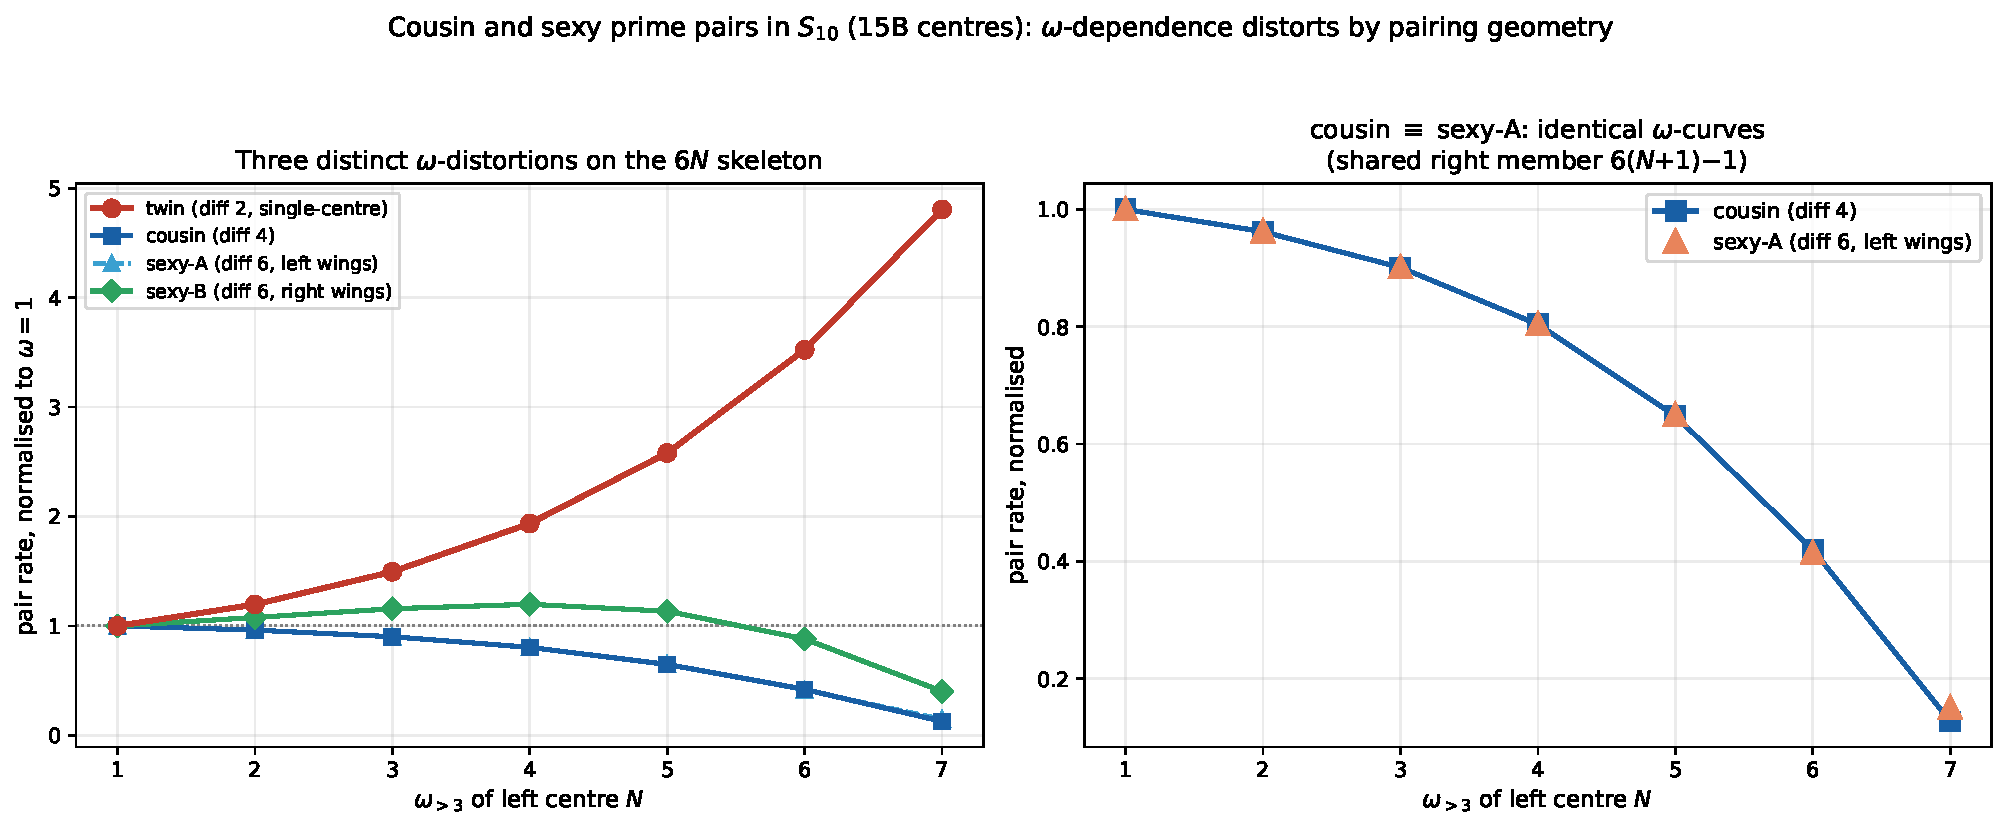
\includegraphics[width=\textwidth]{fig_paper9_cousin_sexy.pdf}
\caption{Left: the three distortions. Twin (red) rises; cousin and sexy-A (blue,
light) fall and overlap; sexy-B (green) is non-monotone. Right: cousin and sexy-A
curves coincide at every $\omega$, explained by their shared right member
$6(N{+}1){-}1$.}
\label{fig:cs}
\end{figure}

\paragraph{Twin: monotone rise.}
The twin reproduces the Parts~II--VIII enrichment: both wings sit on the single
centre $N$, so a factor-rich $N$ protects both, and the rate climbs to $4.8\times$
at $\omega=7$.

\paragraph{Cousin and sexy-A: monotone fall, and identical.}
Both fall to $0.13$--$0.15\times$ at $\omega=7$---opposite to the twin---and they
are numerically equal at every $\omega$ (e.g.\ $0.804$ vs $0.804$ at $\omega=4$,
$0.420$ vs $0.414$ at $\omega=6$). The coincidence has a clean cause: cousin is
$(6N{+}1,6(N{+}1){-}1)$ and sexy-A is $(6N{-}1,6(N{+}1){-}1)$, sharing the right
member $6(N{+}1){-}1$. After normalisation the left member's own $\omega$-response
divides out, leaving the response of the shared right member on the
\emph{adjacent} centre $N{+}1$; that is common to both, so the curves coincide.
The fall (rather than rise) reflects that the right member sits on $N{+}1$, not
$N$: a factor-rich left centre $N$ does not protect a prime on the neighbouring
centre, and the conditioning instead correlates with suppression.

\paragraph{Sexy-B: non-monotone.}
Sexy-B rises to a peak near $\omega=4$ ($1.20\times$) and then falls
($0.40\times$ at $\omega=7$), a third shape distinct from both others. It is the
two-right-wing constellation $(6N{+}1,6(N{+}1){+}1)$, and its non-monotonicity
suggests two competing effects---an early enrichment-like gain and a later
straddle suppression---that we do not separate here.

\section{Discussion and open problem}

The single-centre twin enrichment does not generalise unchanged: once a pair
straddles two consecutive centres, the $\omega$-dependence of the left centre
distorts in a sign and shape fixed by which wings the pair occupies---falling for
cousin and sexy-A (whose conditioned member's partner lives on $N{+}1$),
non-monotone for sexy-B. This is the expected qualitative consequence of the
two-centre geometry that Parts~V--VIII analysed for the twin's own neighbour
correlations, now appearing at leading order because the constellation itself is
two-centred.

\begin{quote}
\textbf{Open problem.} Predict the three curves quantitatively from a two-centre
conditional model over $(N,N{+}1)$, using the modular-shift/lockdown mechanism of
Part~V: the rise of twin, the monotone fall and exact coincidence of cousin and
sexy-A, and the non-monotone peak of sexy-B. A successful model would express
each constellation's $\omega$-curve through the admissibility of its two members
across the two centres.
\end{quote}

\section{Conclusion}

Cousin and sexy prime pairs on the $6N$ skeleton do not inherit the twin's
monotone $\omega$-enrichment. Measured on $S_{10}$, they split into three
geometry-determined shapes: the single-centre twin rises, the straddling
cousin and sexy-A fall and coincide (shared right member), and sexy-B is
non-monotone. The distortion is governed entirely by the pairing geometry---which
centres and which wings---rather than by the difference alone. We report the
phenomenon and its geometric account and leave the quantitative two-centre
mechanism open. As throughout this series, no claim is made about the infinitude
of twin, cousin, or sexy primes, or any $k$-tuple conjecture; this is a measured,
geometry-resolved account of conditional pair rates on the $6N$ skeleton.

\paragraph{Data and code availability.}
The scan and the per-$\omega$ counts are openly available~\cite{repo}; the
$S_{10}$ twin count $23{,}988{,}173$ matches Part~I.

\begin{thebibliography}{9}
\bibitem{ChenI} R.~Chen, \emph{Prime distribution on the $6N$ skeleton} (Part~I),
Zenodo, doi:10.5281/zenodo.20470367 (2026).
\bibitem{ChenII} R.~Chen, \emph{Prime gaps on the $6N$ skeleton} (Part~II),
Zenodo, doi:10.5281/zenodo.20477664 (2026).
\bibitem{ChenV} R.~Chen, \emph{A two-centre shield law} (Part~V), Zenodo,
doi:10.5281/zenodo.20510700 (2026).
\bibitem{ChenVIII} R.~Chen, \emph{The arithmetic structure of the bridge
constant} (Part~VIII), Zenodo, doi:10.5281/zenodo.20519998 (2026).
\bibitem{HL} G.~H.~Hardy, J.~E.~Littlewood, \emph{Partitio Numerorum III}, Acta
Math.\ \textbf{44} (1923), 1--70.
\bibitem{repo} R.~Chen, \emph{$6N$ cousin and sexy prime pairs: data and code},
\url{https://github.com/Ruqing1963/6N-cousin-sexy-distortion} (2026).
\end{thebibliography}

\end{document}
